\documentclass{article}

\usepackage[utf8]{inputenc}
\usepackage{amsmath}
\usepackage{amssymb}
\usepackage{algorithm}
\usepackage[noend]{algpseudocode}
\usepackage{graphicx}
\usepackage{afterpage}
\begin{document}

\title{Exponential Integrators for PDEs arising in meteorology} 
\maketitle
\author{Harvey Sutton}

\tableofcontents
\newpage

\section {Introduction}
%Statement of ODE
It is common within applied mathematics to encounter ODEs of the form
\begin{align}
\dot u(t) = Au(t) + N(u) \label{ODE}
\end{align}
Where $A$ is a large sparse matrix and $N$ denotes some nonlinear term.
As a result, finding accurate approximate solutions to these equations is of major importance.\\

%Method of lines
These ODEs also occure when solving PDEs numerically using the method of lines.
This arrives from discretising the PDE in space yielding an ODE with respect to time, with the form shown in \eqref{ODE}.\\
%ODE Solvers
Soving these ODEs numerically works by progressively stepping through time such as with the explicit forward Euler method, which is given as:
\begin{align*}
u(t+h) &= u(t) + h\dot u(t) = u(t) + h(Au(t) + N(u(t)))
\end{align*}
for a given step size $h$.
%Exponential Integrators
Another method (and the one we will be focusing on here) employs the use of the exponential integrator, which writes the solution to problem \eqref{ODE} over a given time step as:
\begin{align*}
u(t+h) &= e^{Ah}u(t) + \int_0^h e^{A(h-z)}N(u(t+z)) dz \label{ODE Solution}\\
\text{where } e^{A} &= \sum^{\inf}_{i = 0}\frac{A^n}{n!}
\end{align*}
%Computing matrix exponential for A sparse
An important requirement when using this method is to compute approximations of $e^{A}v$ efficiently and accurately for the given sparse matrix $A$ and vector $v$.
One approach would be first to compute $e^A$ and apply the resulting matrix to the vector $v$.
However, even for sparse $A$, $e^{A}$ will likely be dense. For large $A$ this will result in very high memory usage, which may not be practical when approximating solutions to \eqref{ODE Solution}.
One solution to reduce memory usage is to compute $e^{A}v$ directly without computing $e^{A}$ as an intermediary step.\\
Various methods have been proposed for this such as by Al-Mohy, Awad H. and Higham, Nicholas J\cite{AlMohy2011} which is currently used in the Scipy package as \verb|scipy.sparse.linalg.expm_multiply|.
Another class of methods known as Krylov subspace methods have gained traction recently\cite{Moler2003}.
These work by projecting the problem onto a space with fewer dimensions (the kyrlov subspace), computing the matrix exponential and then transforming back to the original space.
As the matrix exponential will be computed in the lower dimension kyrlov subspace the computation cost of this step will not be significant.
\section{Krylov Subspace Methods}
In this section, we will look into existing krylov subspace methods and then compare how these methods perform for approximating $e^{A}v$.

\subsection{Alogrithms}
Here we give the algorithms for the 2 krylov subspace methods we will be comparing.
Each of these algorithms takes a matrix $A\in \mathbb{R}^{n\times n}$, a vector $v \in \mathbb{R}^n$ and an integer $m$ that determines the number of dimensions of the krylov subspace used.
From these algorithms we will get a matrix $H \in \mathbb{R}^{m\times m}$ and another matrix $V \in \mathbb{R}^{n\times m}$ such that $A \approx VHV^T$ and $VV^T = I$.
From here we can get $Av \approx VHV^Tv = VH||v||e_1$.

\begin{algorithm}
\caption{Arnoldi \cite{Fan2018}} %find better citation
\begin{algorithmic}
\Procedure{Arnoldi}{$A, \hat v_1,m$}
\State $v_0 = 0$
\For{$j = 1,2,...,m$}	
\For{$i = 1,2,...,j$}
\State$h_{ij} \gets v_i^T A v_i$
\EndFor
\State$\theta_j \gets Av_j - \sum^j_{i=1} h_{ij}v_i$
\State$h_{j+1,j} \gets ||\theta_j||$
\State$v_{j+1} \gets \theta_j/h_{j+1,j}$
\EndFor
\EndProcedure
\end{algorithmic}
\end{algorithm}
Here V is given by $v_1,...,v_m$ and H is give by $h_1,...,h_m$.\\
\begin{algorithm}
\caption{Lanczos \cite{OJALVO1970}}
\begin{algorithmic}
\Procedure{Lanczos}{$A$ symetric$, \hat v_1,m$}
\State $v_0 = 0$
\For{$i \in \{1,2,...,m\}$}	
\State$\beta_i \gets || \hat v_i ||$
\State$v_i \gets \hat v_i / || \hat v_i ||$
\State$\alpha_i = v_i^T A v_i$
\State$\hat v_{i+1} = Av_i - \alpha_iv_i - \beta_iv_{i-1}$
\EndFor
\EndProcedure
\end{algorithmic}
\end{algorithm}\\
Here $V$ is given by ${v_1,...,v_m}$ and $H$ is tridiagonal with the leading diagonal being $\alpha_1, ..., \alpha_m$ and the upper and lower diagonals being $\beta_2,...,\beta_m$.

\subsection{Relevance To Matrix Exponentials}
By using $A \approx VHV^T$ and the fact that $V^TV = I$ we can apply this to $e^A$ as follows:
\begin{align*}
e^A &= \sum^{\infty}_{i=0}\frac{A^i}{i\!}\\
&= \sum^{\infty}_{i=0}\frac{(VHV^T)^i}{i\!} \\
&= \sum^{\infty}_{i=0}\frac{VH^iV^T}{i\!} \\
&\text {and then when computing $e^Av$ we get}\\
e^Av &= (\sum^{\infty}_{i=0}\frac{VH^iV^T}{i\!})v \\
&= \sum^{\infty}_{i=0}\frac{VH^iV^Tv}{i\!} \\
&= \sum^{\infty}_{i=0}\frac{VH^ie_1}{i\!} \\
&= V(\sum^{\infty}_{i=0}\frac{H^i}{i\!})e_1 \\
&= Ve^He_1
\end{align*}

\subsection{Numerical Results}
Here we run numerical experiments, computing $e^Av$ for a tridiagonal matrix $A$ of sizes $100,000$ and $1,000,000$. We will compare the methods with respect to computation time, error and size of the Kyrlov subspace.

\begin{figure}

    \centering
    \begin{minipage}{0.5\textwidth}
       \centering
	  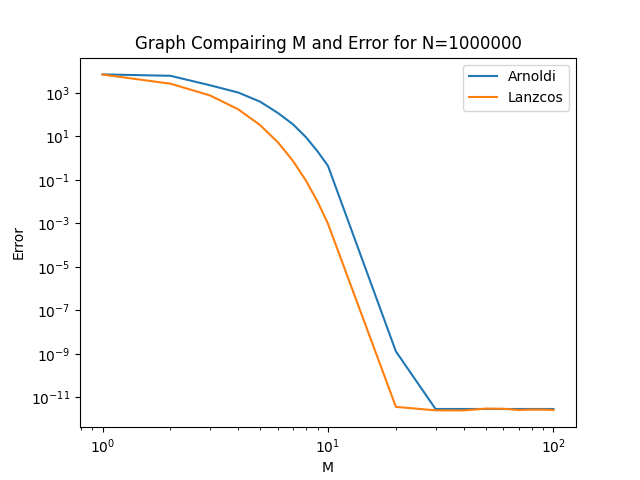
\includegraphics[width=\linewidth]{Plots/M v E Results for N=1000000.png}
	  \label{fig:MEe7}
       \centering
	  \includegraphics[width=\linewidth]{Plots/M v Comp Time Results for N=1000000.png}
	  \label{fig:MEe7}
       \centering
	  \includegraphics[width=\linewidth]{Plots/Comp Time v E Results for N=1000000.png}
	  \label{fig:MEe7}
    \end{minipage}\hfill
    \begin{minipage}{0.5\textwidth}
       \centering
	  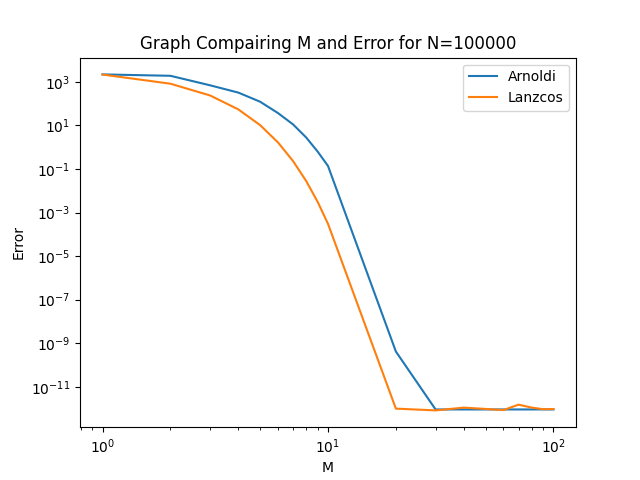
\includegraphics[width=\linewidth]{Plots/M v E Results for N=100000.png}
	  \label{fig:MEe6}
       \centering
	  \includegraphics[width=\linewidth]{Plots/M v Comp Time Results for N=100000.png}
	  \label{fig:MEe6}
       \centering
	  \includegraphics[width=\linewidth]{Plots/Comp Time v E Results for N=100000.png}
	  \label{fig:MEe6}
    \end{minipage}
These results show that the Lanzcos algorithm outperforms the Arnoldi algorithm in both convergence rate and computational time.
\end{figure}

\begin{figure}
Below we compare the time required for the different algorithms to get below an error of $10^{10}$ when computing $e^Av$ for various matrix sizes.
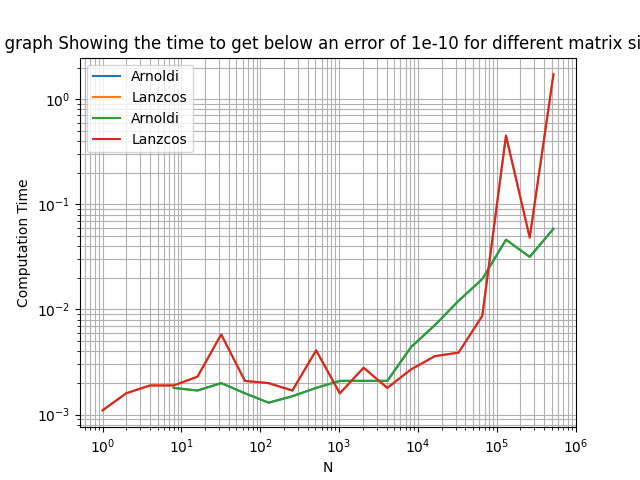
\includegraphics[width=\linewidth]{Plots/time to get below an error of 1e-10.png}
\clearpage
Again we continue to see that the Lanzcos algorithm outperforms the Arnodli algorithm.
\end{figure}
\clearpage
\newpage
\bibliographystyle{plain}
\bibliography{References.bib}

\end{document}